 
\def\filename{leaflet-manual.tex}
\def\fileversion{v1.0d}   % change this when leaflet-manual changed, too.
\def\filedate{2012/06/04}
\def\docdate {2012/06/04} % change this when leaflet-manual changed, too.
\listfiles
\errorcontextlines=99
\documentclass[
notumble,
nofoldmark,
%%dvipdfm,
%%portrait,
%%titlepage,
%%nocombine,
%%a3paper,
%%debug,
%%nospecialtricks,
%%draft,
]{leaflet}
\setmargins{15mm}{8mm}{12mm}{12mm}
% \usepackage[widht=311mm,height=214mm,center]{crop}
\usepackage{tabularx}
\usepackage{lipsum}
\usepackage{eurosym}
\renewcommand*\foldmarkrule{.3mm}
\renewcommand*\foldmarklength{5mm}

\usepackage[T1]{fontenc}
% \usepackage[T3]{inputenc}
\usepackage{textcomp}
\usepackage{mathptmx}
\usepackage{libertine}
% \usepackage[scaled=0.9]{helvet}
\makeatletter
\def\ptmTeX{T\kern-.1667em\lower.5ex\hbox{E}\kern-.075emX\@}
\DeclareRobustCommand{\ptmLaTeX}{L\kern-.3em
        {\setbox0\hbox{T}%
         %\vb@xt@ % :-)
         \vbox to\ht0{\hbox{%
                            \csname S@\f@size\endcsname
                            \fontsize\sf@size\z@
                            \math@fontsfalse\selectfont
                            A}%
                      \vss}%
        }%
        \kern-.12em
        \ptmTeX}
\makeatother
\let\TeX=\ptmTeX
\let\LaTeX=\ptmLaTeX
\usepackage{shortvrb}
\MakeShortVerb{\|}
\usepackage{url}
\usepackage{graphicx}
\usepackage[dvipsnames,usenames]{color}
\usepackage[table]{xcolor}

 
\usepackage{fontspec}

\setsansfont[
	%Ligatures={TeX,Common},		% not supported by ttf
	Scale=MatchLowercase,
% 	Path=\fontpath,
	BoldFont = Arimo-Bold_B.ttf ,
	ItalicFont = Arimo-Italic_B.ttf ,				
	BoldItalicFont = Arimo-BoldItalic_B.ttf 		
	]{Arimo_B.ttf}


\usepackage{titlesec}

\setmargins{10mm}{8mm}{12mm}{12mm}

\titleformat*{\section}{\color{LIGHTGRAY} \sffamily \Large }


\definecolor{LIGHTGRAY}{gray}{.9}
\definecolor{lspblue1}{cmyk}{0.9,0.4,0.05,0}
\definecolor{langscicol1}{cmyk}{0.6,0.05,0.05,0}
\definecolor{langscicol2}{cmyk}{0.75,0.15,0,0}
\definecolor{langscicol3}{cmyk}{0.9,0.4,0.05,0}
\definecolor{langscicol4}{cmyk}{0.9,0.5,0.15,0.3}
\definecolor{langscicol5}{cmyk}{1,0.47,0.22,0.68}
\definecolor{langscicol6}{cmyk}{0,0.25,1,0}
\definecolor{langscicol7}{cmyk}{0,0.50,1,0}
\definecolor{langscicol8}{cmyk}{0,0.64,1,0}
\definecolor{langscicol9}{cmyk}{0,0.78,1,0}
\definecolor{langscicol10}{cmyk}{0.05,1,0.8,0}
\definecolor{langscicol11}{cmyk}{0.3,1,0.6,0}
\definecolor{langscicol12}{cmyk}{0.54,1,0.65,0.1}
\definecolor{langscicol13}{cmyk}{0.58,1,0.70,0.35}
\definecolor{langscicol14}{cmyk}{0.32,0.02,0.72,0}
\definecolor{langscicol15}{cmyk}{0.4,0,1,0}
\definecolor{langscicol16}{cmyk}{0.55,0,0.9,0.1}
\definecolor{langscicol17}{cmyk}{0.6,0,0.9,0.35}
\definecolor{langscicol18}{cmyk}{0.85,0.02,0.95,0.38}
\definecolor{langscicol19}{cmyk}{0.85,0.05,1,0.5}
\definecolor{langscicol20}{cmyk}{0.88,0.15,1,0.66}

\definecolor{lsLightBlue}{cmyk}{0.6,0.05,0.05,0}
\definecolor{lsMidBlue}{cmyk}{0.75,0.15,0,0}
\definecolor{lsMidDarkBlue}{cmyk}{0.9,0.4,0.05,0}
\definecolor{lsDarkBlue}{cmyk}{0.9,0.5,0.15,0.3}
\definecolor{lsNightBlue}{cmyk}{1,0.47,0.22,0.68}
\definecolor{lsYellow}{cmyk}{0,0.25,1,0}
\definecolor{lsLightOrange}{cmyk}{0,0.50,1,0}
\definecolor{lsMidOrange}{cmyk}{0,0.64,1,0}
\definecolor{lsDarkOrange}{cmyk}{0,0.78,1,0}
\definecolor{lsRed}{cmyk}{0.05,1,0.8,0}
\definecolor{lsLightWine}{cmyk}{0.3,1,0.6,0}
\definecolor{lsMidWine}{cmyk}{0.54,1,0.65,0.1}
\definecolor{lsDarkWine}{cmyk}{0.58,1,0.70,0.35}
\definecolor{lsSoftGreen}{cmyk}{0.32,0.02,0.72,0}
\definecolor{lsLightGreen}{cmyk}{0.4,0,1,0}
\definecolor{lsMidGreen}{cmyk}{0.55,0,0.9,0.1}
\definecolor{lsRichGreen}{cmyk}{0.6,0,0.9,0.35}
\definecolor{lsDarkGreen1}{cmyk}{0.85,0.02,0.95,0.38}
\definecolor{lsDarkGreen2}{cmyk}{0.85,0.05,1,0.5}
\definecolor{lsNightGreen}{cmyk}{0.88,0.15,1,0.66}

% \usepackage{langscicolors}
%%%%\renewcommand{\descfont}{\normalfont}
\newcommand\Lpack[1]{\textsf{#1}}
\newcommand\Lclass[1]{\textsf{#1}}
\newcommand\Lopt[1]{\texttt{#1}}
\newcommand\Lprog[1]{\textit{#1}}

\newcommand*\defaultmarker{\textsuperscript\textasteriskcentered}

\newcommand{\lsptable}[2]{
\begin{tabularx}{#1}{XXXXXXXXXXXXXXXXXXXX}
\cellcolor{langscicol1}
&
\cellcolor{langscicol2}
&
\cellcolor{langscicol3}
&
\cellcolor{langscicol4}
&
\cellcolor{langscicol5}
&
\cellcolor{langscicol6}
&
\cellcolor{langscicol7}
&
\cellcolor{langscicol8}
&
\cellcolor{langscicol9}
&
\cellcolor{langscicol10}
&
\cellcolor{langscicol11}
&
\cellcolor{langscicol12}
&
\cellcolor{langscicol13}
&
\cellcolor{langscicol14}
&
\cellcolor{langscicol15}
&
\cellcolor{langscicol16}
&
\cellcolor{langscicol17}
&
\cellcolor{langscicol18}
&
\cellcolor{langscicol19}
&
\cellcolor{langscicol20}
\rule{0pt}{#2}
\end{tabularx}

}

\title{Language Science Press}
\author{%
  Sebastian Nordhoff}
\date{Last updated~\docdate\\printed \today} 
% \CutLine*{1}% Dotted line without scissors
% \CutLine*{6}%   

% \AddToBackground{5}{%  Background of a small page
%   \put(0,0){\textcolor{Cerulean}{\rule{\paperwidth}{\paperheight}}}}
\AddToBackground*{1}{%  Background of a small page
  \put(0,0){\textcolor{lspblue1}{\rule{\paperwidth}{\paperheight}}}}
\AddToBackground*{2}{%  Background of a small page
  \put(0,0){\textcolor{lspblue1}{\rule{\paperwidth}{\paperheight}}}}

% \AddToBackground*{2}{% Background of a large page
%   \put(\LenToUnit{.5\paperwidth},\LenToUnit{.5\paperheight}){%
%     \makebox(0,0)[c]{%
%       \resizebox{.9\paperwidth}{!}{\rotatebox{35.26}{%
%         \textsf{\textbf{\textcolor{LIGHTGRAY}{BACKGROUND}}}}}}}}

\AddToBackground{2}{
    \put(-20,600){
%         
\includegraphics[width=3\paperwidth]{lsp-rainbow-large.png}%
 \setlength{\tabcolsep}{0pt} 
% \resizebox{3.1\paperwidth}{.5cm}{\lsptable{\paperwidth}{5.5cm}}
    } 
}

% \AddToBackground{5}{
%     \put(-2,-100){
%         
\includegraphics[width=3\paperwidth]{lsp-rainbow-large.png}%
% %  \setlength{\tabcolsep}{0pt}
% % 	\begin{tabularx}{3\paperwidth}{X|X|X|X|X|X|X|X|X|X|X|X|X|X|X|X|X|X|X}
% % &&&&&&&&&&&&&&&&&&
% % \end{tabularx}
%     } 
% }


\AddToBackground{6}{
    \put(277,580){
	\lsptable{\paperwidth}{1.5cm}
%         
\includegraphics[width=1\paperwidth,height=3.5cm]{lsp-rainbow-large.png}%
    } 
}


\AddToBackground{6}{
    \put(427,28){ 
{\color{white}
\includegraphics[width=4cm]{langsci_logo_nocolor.pdf}  }
%         
\includegraphics[width=1\paperwidth,height=3.5cm]{lsp-rainbow-large.png}%
    } 
}

\AddToBackground{2}{
    \put(-5,13){    
% 	\resizebox{.5\paperwidth}{.5cm}{\lsptable{\paperwidth}{5.5cm}}
%         
\includegraphics[width=.3\paperwidth]{lsp-rainbow-large.png}%
    } 
}

% \AddToBackground{3}{
%     \put(-2,10){
%         
\includegraphics[width=.3\paperwidth]{lsp-rainbow-large.png}%
%     } 
% }

% \AddToBackground{4}{
%     \put(-2,10){
%         
\includegraphics[width=.3\paperwidth]{lsp-rainbow-large.png}%
%     } 
% }

\setlength{\itemsep}{-3pt}
\usepackage{enumitem}
\setlist[itemize]{leftmargin=-0em}
 \usepackage{titlesec}
\titlespacing*{\section}
  {0pt}{\baselineskip}{0pt}
\begin{document}

% \maketitle
\thispagestyle{empty}

%%\LARGE
\color{LIGHTGRAY}
%%\tableofcontents

 
\vspace*{2cm}
\resizebox{\textwidth}{!}{
  \parbox{.32\textwidth}{ 
  \large\sffamily \parbox[t][.2cm][t]{3cm}{Language} \\[-.2em]
  \parbox[t][.2cm][t]{3cm}{Science} \\[-.2em]
  \parbox[t][.2cm][t]{3cm}{Press} \\[-.3em]
   \resizebox{1.5cm}{!}{\rmfamily \tiny Open Access Monographs} 
  }
}
  

    


\newpage


\vspace*{-1.5cm}
% 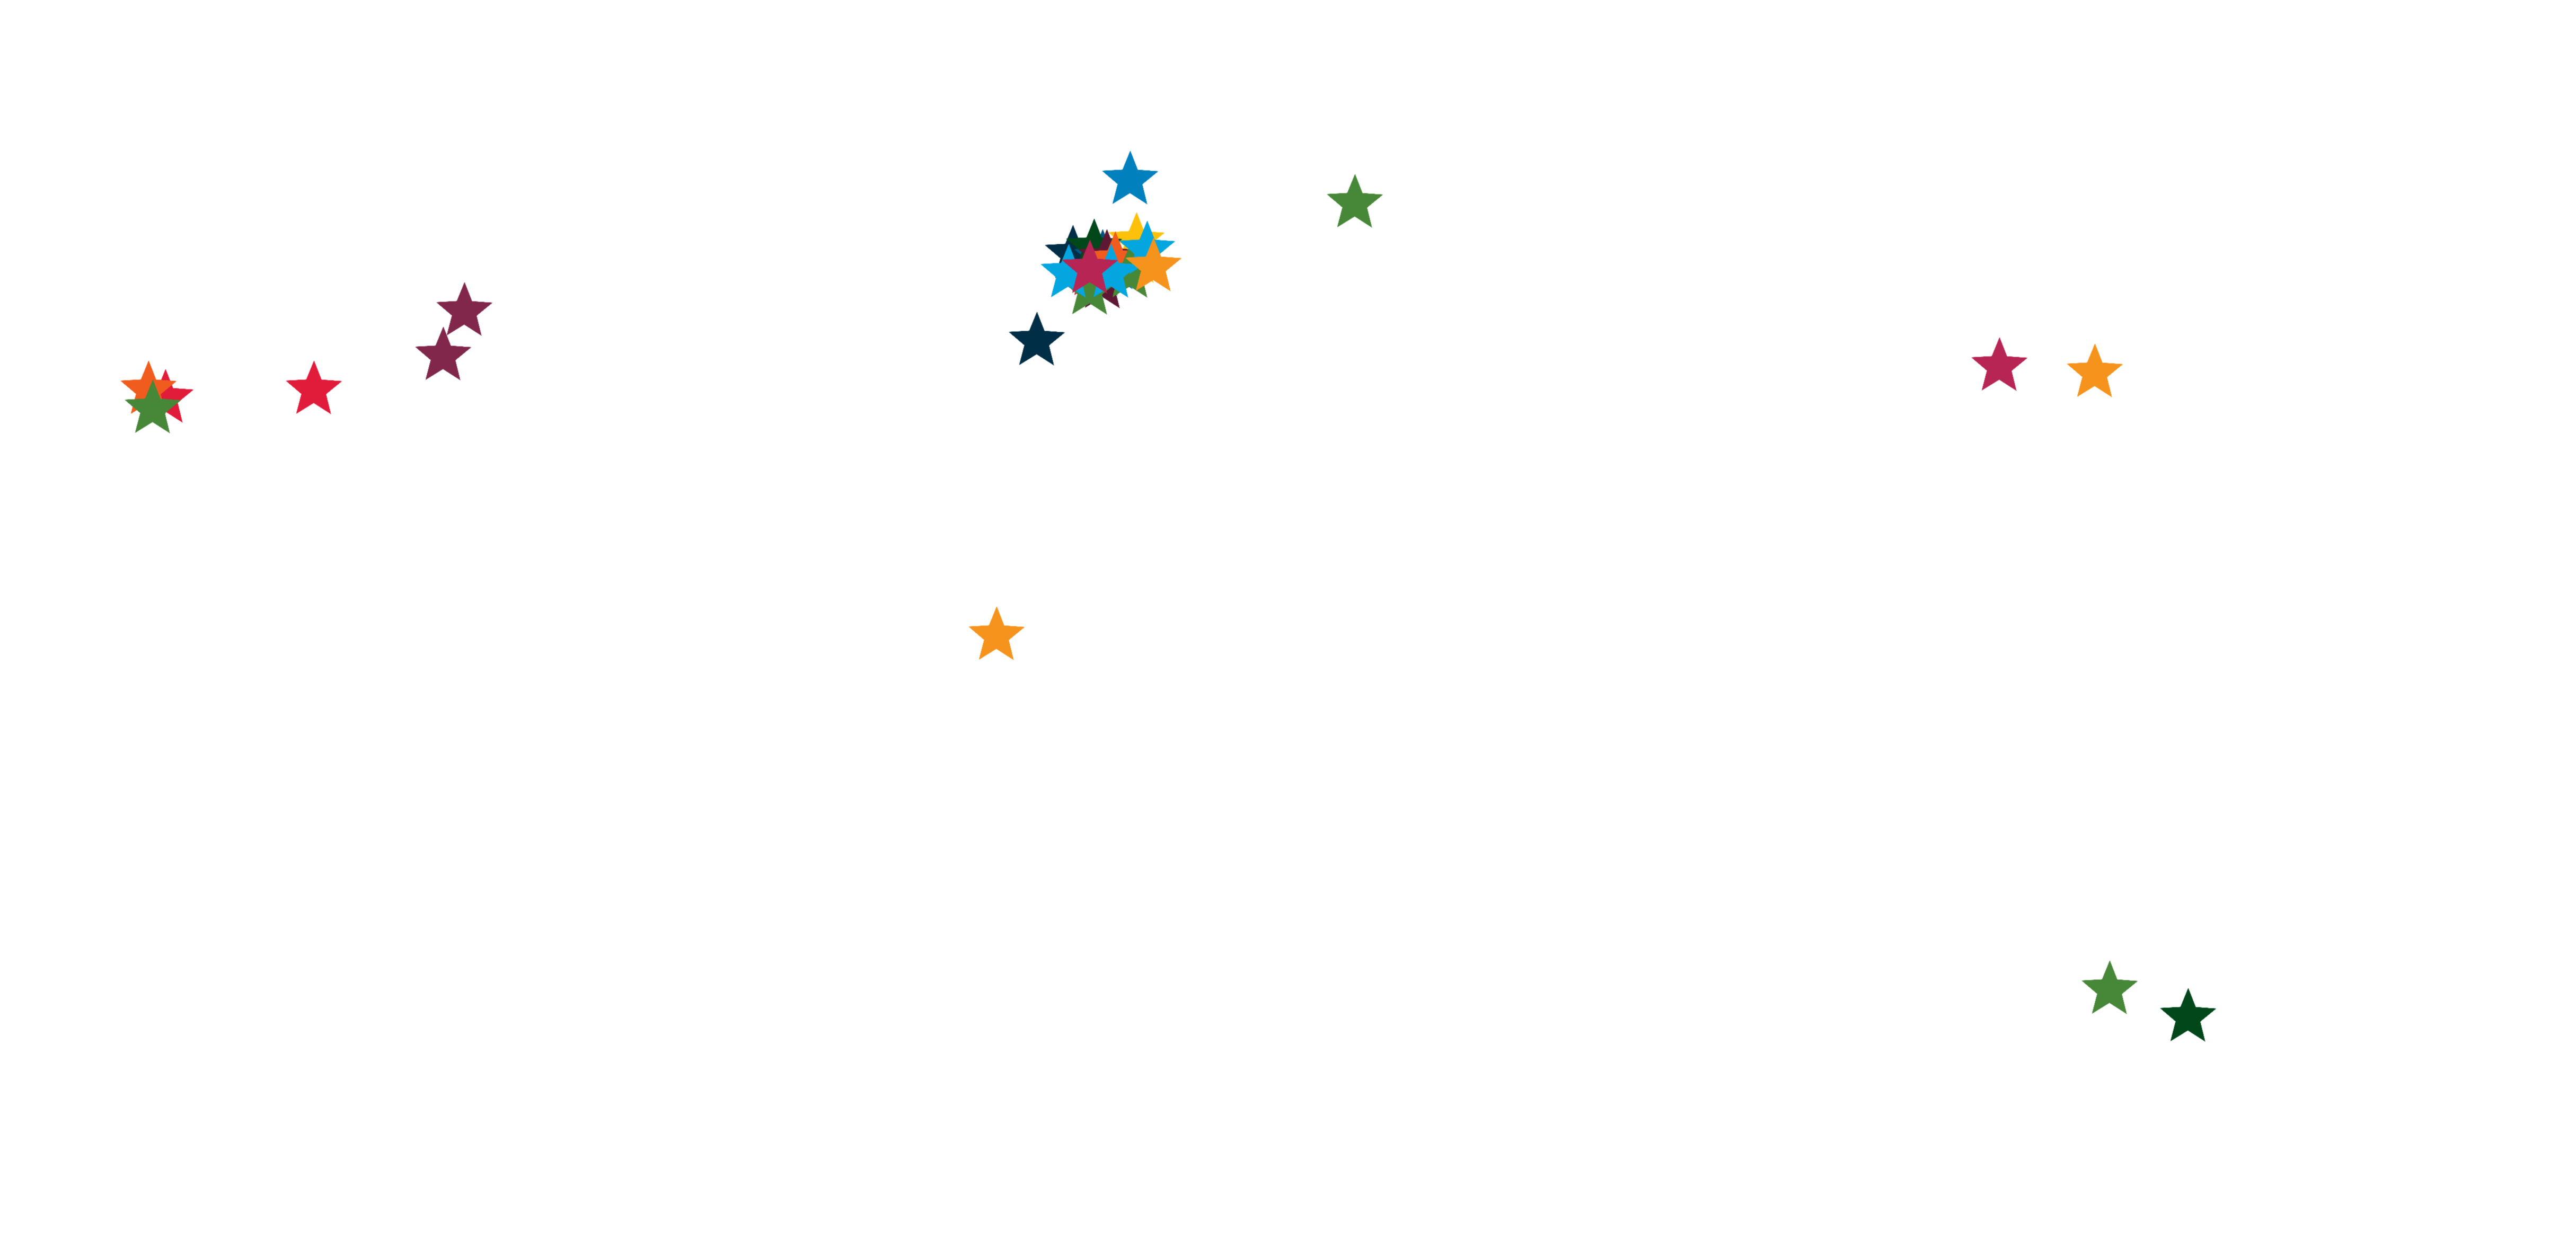
\includegraphics[width=2.6\textwidth]{worldmapdots2.png}
% 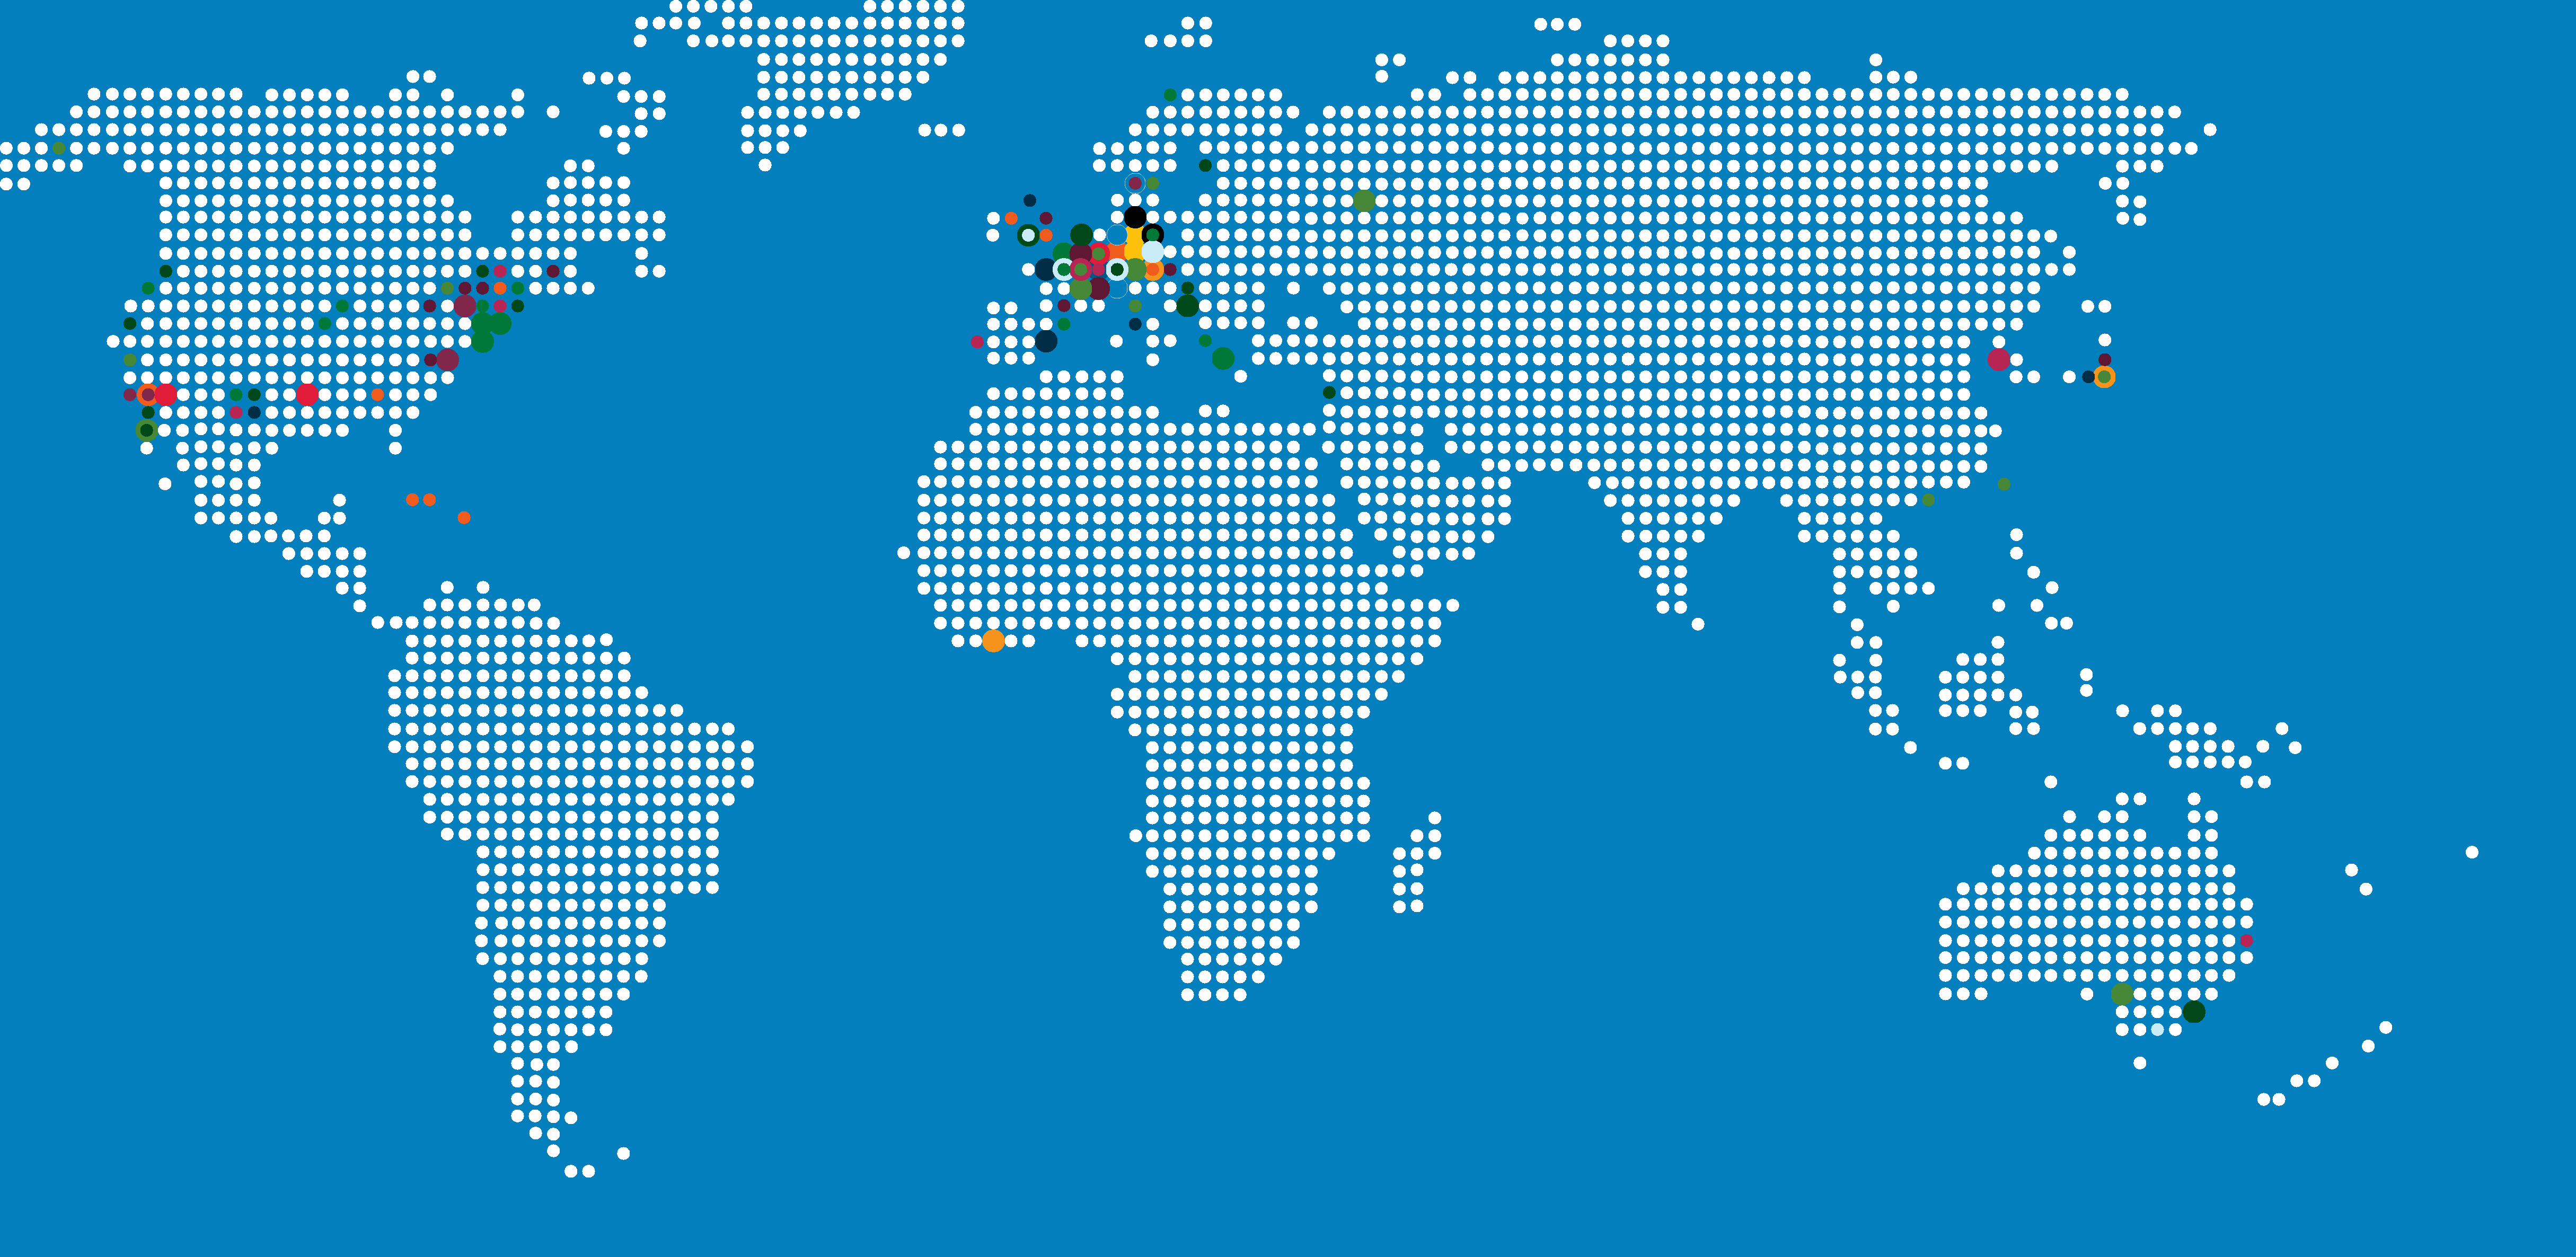
\includegraphics[width=2.6\textwidth]{WORLDMAPDOTSdots.png}
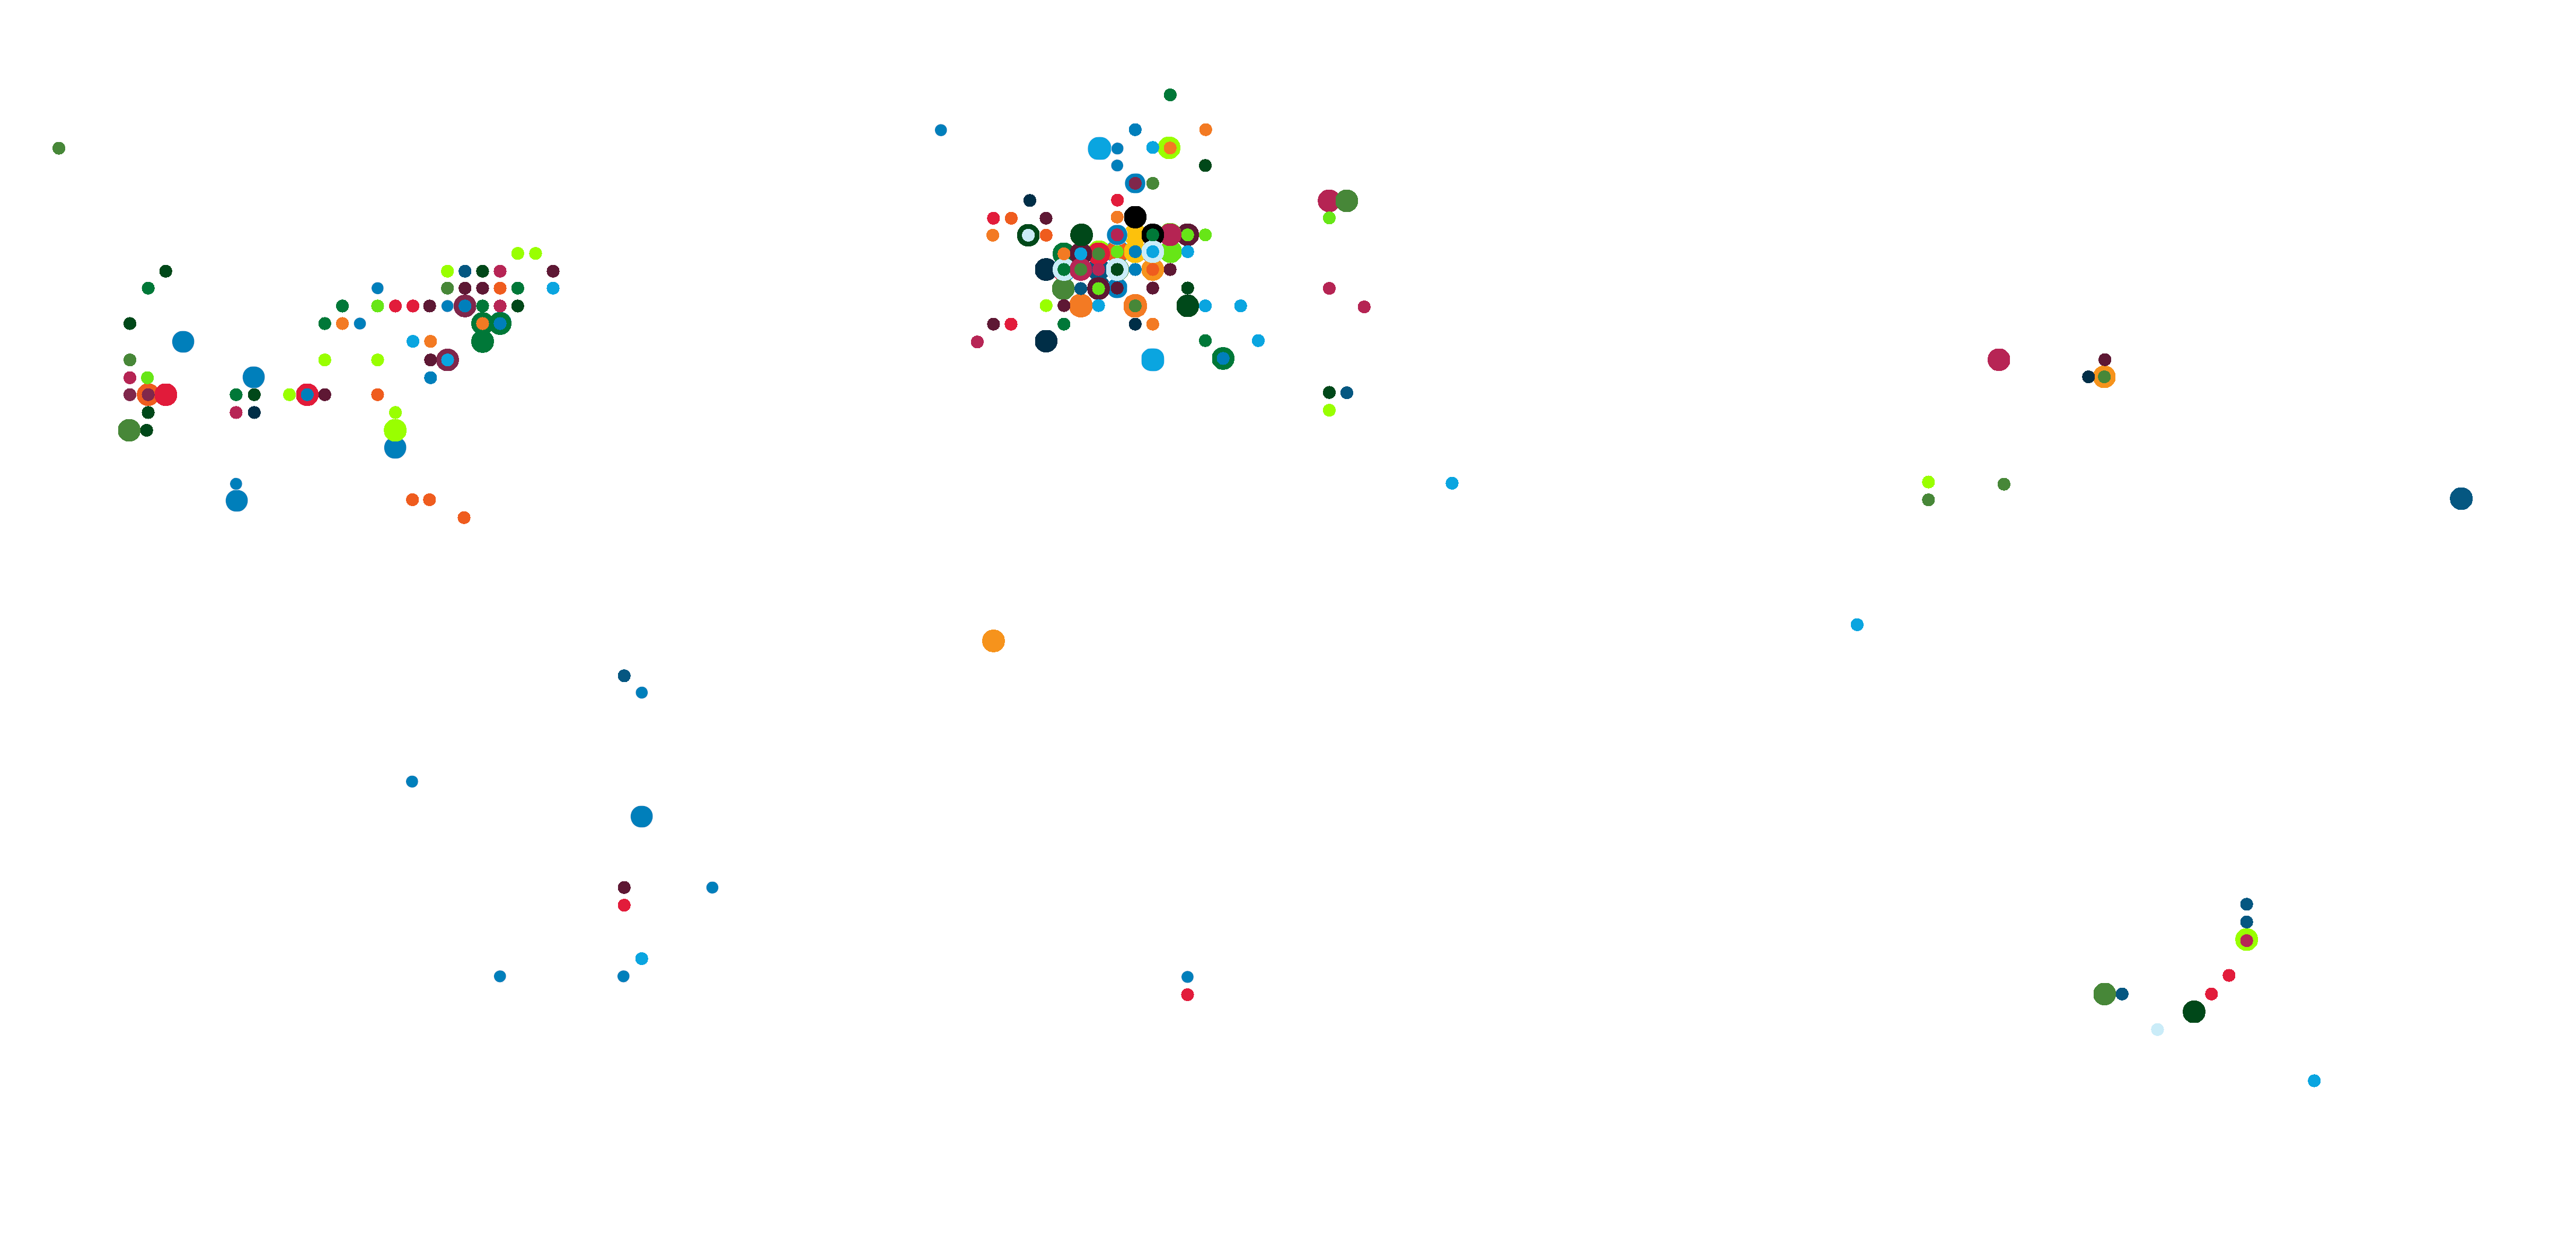
\includegraphics[width=2.6\textwidth]{WORLDMAPDOTSlargedots.png}

\vspace*{-20mm}
\section{\sffamily\Large\bfseries Series}

% \newcommand{\series}[3]{   
%   \parbox{.1\textwidth}{~}
%   \parbox{.7\textwidth}{\raggedleft\small #1\\{\scriptsize #3}}
%   \parbox{.1\textwidth}{\includegraphics[width=.8cm]{#2.png}} 
% }
% 
% \newcommand{\series}[3]{   
%   \parbox{.1\textwidth}{~}
%   \parbox{.7\textwidth}{\raggedleft\small #1\\{\scriptsize #3}}
%   \parbox{.1\textwidth}{\includegraphics[width=.8cm]{#2.png}} 
% }

\newcommand{\series}[3]{   
  \parbox{.1\textwidth}{\includegraphics[width=.6cm]{#2.png}}
  \parbox{.01\textwidth}{~} 
  \parbox{.7\textwidth}{\raggedright{\small\bfseries #1}\\{\scriptsize #3}}
  \parbox{.05\textwidth}{~\smallskip}\\[.5em]
} 

\series{African Language Grammars and Dictionaries}{algad}{Adams Bodomo, Ken Hiraiwa, Firmin Ahoua}
\series{Classics in Linguistics}{classics}{\mbox{Stefan Müller, Martin Haspelmath}}
\series{Computational Models of Language Evolution}{cmle}{Luc Steels, Remi van Trijp}
\series{Conceptual Foundations of Language Science}{cfls}{Mark Dingemanse, Nick Enfield}
\series{Contemporary African Linguistics}{cal}{Lee Bickmore, Akinbiyi Akinlabi}
\series{Empirically Oriented Theoretical Morphology and Syntax}{eotms}{\mbox{Stefan M\"uller, Berthold Crysmann, Laura Kallmeyer}}
\series{EuroSLA studies}{eurosla}{Gabriele Pallotti} 
\series{Language Variation}{lv}{John Nerbonne, Dirk Geeraerts}
\series{\mbox{Monographs on Comparative Niger-Congo}}{mcnc}{Valentin Vydrin, Larry Hyman, Konstantin Pozdniakov, Guillaume Segerer, John Watters}
 

   
\vspace*{7.72cm} 
\series{\mbox{Morphological Investigations}}{mi}{\mbox{James P. Blevins, Petar Milin, Michael Ramscar}}
\series{Open Generative Syntax}{ogs}{Elena Anagnostopoulou, Mark Baker, Roberta D’Alessandro, David Pesetsky, Susi Wurmbrand}
\series{Phraseology and Multiword Expressions}{pmwe}{Manfred Sailer, Agata Savary}
\series{Studies in Caribbean Languages}{scl}{John R. Rickford, Joseph Farquharson}
\series{Studies in Diversity Linguistics}{sidl}{Martin Haspelmath, Fernando Z\'u\~niga, Peter Arkadiev, Ruth Singer, Pilar Valenzuela}
\series{Studies in Laboratory Phonology}{silp}{Martine Grice, Doris M\"ucke, Taehong Cho}
\series{Textbooks in Language Sciences}{tbls}{\mbox{Stefan M\"uller, Martin Haspelmath, Claude Hag\`ege,} \mbox{Marianne Mithun, Anatol Stefanowitsch, Foong Ha Yap}}	 
\series{\mbox{Topics at the Grammar-Discourse Interface}}{tgdi}{\mbox{Philippa Cook, Anke Holler, Cathrine Fabricius-Hansen}}
\series{Translation and Multilingual Natural Language Processing}{tmnlp}{{Oliver \v{C}ulo, Silvia Hansen-Schirra,   Reinhard Rapp}}
  
      
\newpage
\section{\sffamily\Large\bfseries About}
\begin{itemize}  
\setlength{\itemsep}{-3pt} 
 \item[›] Language Science Press is a scholar-owned press
 \item[›]  High quality, peer-reviewed open-access books in linguistics
  \item[›] Currently 18 series with editorial board members from all over the world
 \item[›] Published under a Creative Commons licence
 \item[›] Free for both authors and readers
%  \item[›] General Editors are Stefan M\"uller (FU Berlin) and Martin Haspelmath (MPI for Evolutionary Anthropology)
%  \item[›] Supported by a high-profile Advisory Board
 \item[›] Supported by the DFG with 500k{\euro} during the startup phase

 \item[›] All books appear in a book series, and the series editors are responsible for acquiring, reviewing and selecting manuscripts for publication
%  \item[›] The authors are responsible for typesetting in LaTeX (together with the series editors); automatic conversion from Word is possible in principle.
 \item[›] Online workflow based on the publication management system Open Monograph Press
 \item[›] Pdfs are available free of charge from our website 
 \item[›] Printed copies can be ordered from our print-on-demand partners
%  \item[›] 
%  \item[›] 
%  \item[›] 
\end{itemize}
 
 \section{\sffamily\Large\bfseries Philosophy} 
 For some time now, all scholars have been accustomed to sharing their materials at no cost with their colleagues, often with the help of services like Academia.edu and ResearchGate. Scientific publication thus no longer serves the need of disseminating research results -- its purpose is to make the best work prominent enough to help build careers and to guide scholars in choosing what to read. This task of selecting the best work is carried out by the series editors of Language Science Press.

 Our philosophy is that book publishing can be fully under the control of scholars because most of the traditional tasks of commercial publishers can be done more efficiently by scholars. 
 
As of December 2016, more than 220 scholars have proposed manuscripts to Language Science Press. For the latest publications, see our website www.langsci-press.org. 
   
\newpage 
\newlength{\submissionfactor}
\setlength{\submissionfactor}{.5mm}
\newcommand{\submission}[3]{
\parbox[m][.1cm][c]{2.5cm}{\color{LIGHTGRAY} #1}\colorbox{#2}{\parbox[m][.3cm][c]{#3\submissionfactor}{\bfseries\sffamily #3}}\\ 
}

\section{\sffamily\Large\bfseries Submissions}
\submission{desk rejection}{lsRed}{28}
\submission{in preparation}{lsLightBlue}{118}
\submission{under review}{lsDarkBlue}{6}
\submission{rejected}{lsLightOrange}{10}
\submission{forthcoming}{lsSoftGreen}{22}
\submission{published}{lsRichGreen}{27}

% \color{LIGHTGRAY}
% \begin{tabular}{ll}
% desk rejection & \colorbox{lsRed}{\parbox{12mm}{15}}\\
% in preparation &  \colorbox{lsLightBlue}{\parbox{30mm}{34}}\\
% under review & \colorbox{lsDarkBlue}{\parbox{6mm}{7}} \\
% rejected & \colorbox{lsLightWine}{\parbox{3mm}{4}} \\
% forthcoming &  \colorbox{lsMidGreen}{\parbox{14mm}{13}}\\
% published & \colorbox{lsRichGreen}{\parbox{6mm}{9}} \\
% \end{tabular}


 


\section{\sffamily\Large\bfseries Downloads}
\vspace*{-1em}
% 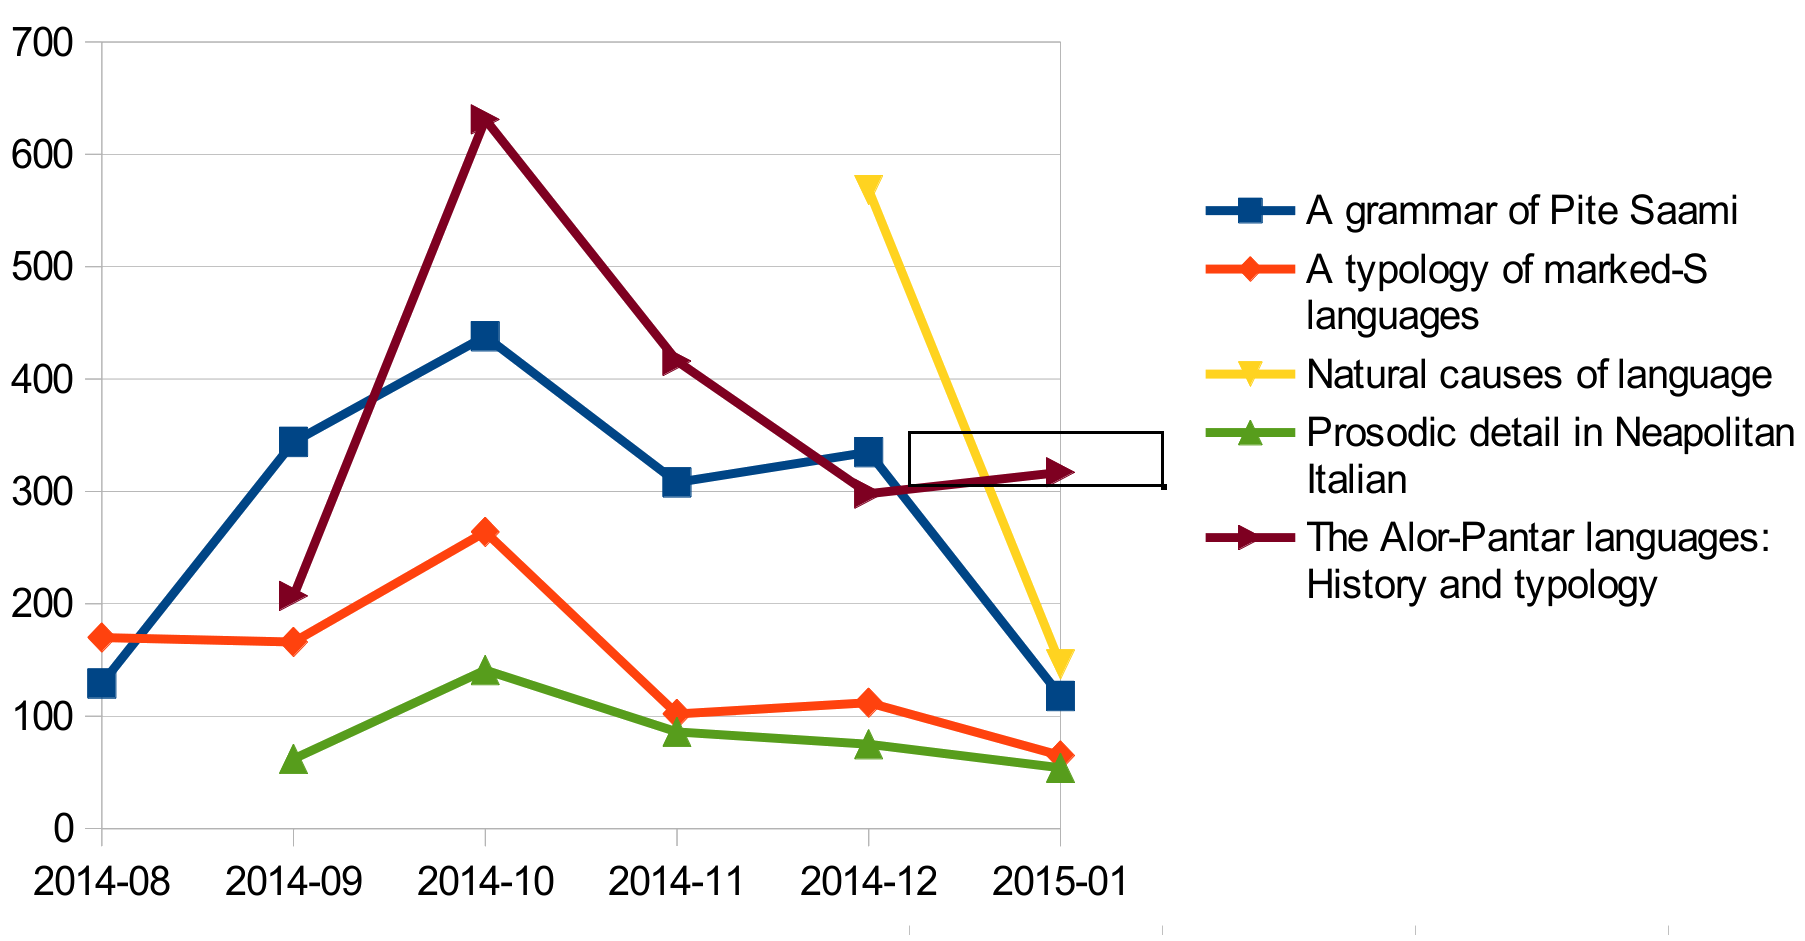
\includegraphics[width=\textwidth]{statistiks.png}
\parbox[b][0cm][b]{0cm}{
\raisebox{0cm}{
\hspace{.7\textwidth}\tiny\color{LIGHTGRAY} Numbers as of 2016-12-31
}
}

\setlength{\tabcolsep}{0pt}
\newlength{\downloadfactor}
\setlength{\downloadfactor}{.7mm}
\newcommand{\downloadbox}[4]{\begin{tabular}{p{#1.#2\downloadfactor}}\cellcolor{#3}\sffamily\bfseries~#1#2\rule{0pt}{1.5em}\\\mbox{#4}\end{tabular}\\[.1em]
\\}

\resizebox{2\textwidth}{!}{
\sffamily
\color{LIGHTGRAY}
\noindent
  \parbox{19cm}{
    \downloadbox{156}{43}{lsMidWine}{The future of dialects}
    \downloadbox{112}{74}{lsYellow}{Einführung in die grammatische Beschreibung des Deutschen}
    \downloadbox{98}{85}{lsRichGreen}{The Alor-Pantar languages}
    \downloadbox{90}{72}{lsDarkBlue}{New directions in corpus-based translation studies}
    \downloadbox{82}{12}{lsYellow}{Grammatical theory}    
  }
} 

\vspace*{-1em}
% 
\section{\sffamily\Large\bfseries Support us!}
  
\color{LIGHTGRAY}
    \begin{itemize}
\setlength{\itemsep}{-3pt} 
      \item[›] submit your manuscript to one of the series
      \item[›] start a series for your subfield of linguistics
      \item[›] become a community proofreader 
      \item[›] become a community typesetter
      \item[›] become a public supporter
      \item[›] donate
      \item[›] have your library support us via Knowledge\\ Unlatched
    \end{itemize} 


  
 

\newpage 
\color{LIGHTGRAY}
\section{\sffamily\Large\bfseries Advisory Board}

\begin{itemize}
\setlength{\itemsep}{-3pt} 
 \item[›] Artemis Alexiadou (Stuttgart)
 \item[›] Jim Blevins (Cambridge)
 \item[›] Balthasar Bickel (Z\"urich)
 \item[›] Geert Booij (Leiden)
 \item[›] Miriam Butt (Konstanz)
 \item[›] Ewa D\k{a}browska (Northumbria)
 \item[›] Arnulf Deppermann (IDS Mannheim)
 \item[›] Nomi Erteschik-Shir (Ben Gurion)
 \item[›] Martine Grice (Cologne)
 \item[›] Mutsumi Imai (Tokyo)
 \item[›] Laura Kallmeyer (D\"usseldorf)
 \item[›] Manfred Krifka (Berlin)
 \item[›] Mary Esther Kropp Dakubu (Accra)
 \item[›] Aditi Lahiri (Oxford)
 \item[›] Stephen Levinson (MPI Nijmegen)
 \item[›] Anke L\"udeling (Berlin)
 \item[›] Detmar Meurers (T\"ubingen)
 \item[›] Sam Mchombo (Berkeley)
 \item[›] Rachel Nordlinger (Melbourne)
 \item[›] Jairo Nunes (S\~ao Paulo)
 \item[›] Steven Pinker (Harvard)
 \item[›] Friedemann Pulverm\"uller (Berlin)
 \item[›] Stuart Shieber (Harvard)
 \item[›] Dieter Stein (D\"usseldorf)  
\end{itemize}

\section{\sffamily\Large\bfseries Contact}  

\setlength{\tabcolsep}{0pt}
\begin{tabular}{ll}
 
% \begin{tabular}{p{.6\textwidth}l} 
\parbox{.64\textwidth}{www.langsci-press.org\\
contact@langsci-press.org\\
@langscipress \\
\\
Stefan M\"uller 
{\\\scriptsize Press Director}
\\
Martin Haspelmath
{\\\scriptsize Press Director}\\
Sebastian Nordhoff  
{\\\scriptsize Coordinator}
}&
\\%[-1em]
&
\parbox[b][0cm][b]{0cm}{
\includegraphics[width=.35\textwidth]{qrcode.eps}  
}
\end{tabular}
% Stefan M\"uller \\
% Martin Haspelmath\\
% Sebastian Nordhoff  
% }

 



% \framebox[3cm]{ \textbf{Mitmachen?}\\ Author\par Editor}




% \fbox{
% \textbf{Mitmachen?}
% \\
% Author
% \\
% Editor
% \\
% Proofreader
% \\
% Typesetter
% \\
% Membership
% \\
% Donate
% 
% }

% \begin{itemize}
%  \item[›] autor
% \item[›] hrsg
% \item[›] proofreader
% \end{itemize}
 

\loggingall
\end{document}
\endinput
%%
%% End of file `leaflet-manual.tex'.
